\documentclass{beamer}
\usetheme{Frankfurt}

\usepackage[utf8]{inputenc}
\usepackage{physics}
\usepackage{makecell}
\usepackage{tikz-cd}
\usepackage{wasysym} 
\usepackage{tikz}
\usepackage{xcolor}

\setbeamertemplate{navigation symbols}{}

\DeclareMathOperator{\id}{id}
\DeclareMathOperator{\diag}{diag}
\DeclareMathOperator{\Span}{span}
\DeclareMathOperator{\Aut}{Aut}

\title[Tomita-Takesaki and Quantum]{Applications of Tomita-Takesaki Theory to Quantum Physics I\nocite{Burbano2017}}
\subtitle{Canonical Dynamics Induced by States in Thermal Equilibrium}
\author[Iván Burbano]{Iván Mauricio Burbano Aldana}
\institute{Universidad de los Andes}
\date{\today}

\begin{document}

\begin{frame}
	\titlepage
\end{frame}

\begin{frame}
	\frametitle{Motivation}
	\begin{columns}
		\column{0.5\textwidth}
		\includegraphics[width=\textwidth]{images/pendulum.png}
		\column{0.5\textwidth}
		Can we obtain the equations of motion from the equilibrium state?
		\vspace{1cm}
		
		\onslide<2->{Maybe in quantum thermal systems.
		\begin{align*}
			e^{-\beta H} &\circlearrowright e^{-iHt} \\
			\text{temperature} &\iff i\times\text{time}
		\end{align*}}
	\end{columns}
\end{frame}

\begin{frame}
	\tableofcontents
\end{frame}

\section{Operator Theory and Physics}

\begin{frame}
	
	\frametitle{Classical and Quantum Theories}

	\begin{table}
	\begin{tabular}{|c|c|c|}
	\hline
	& Classical & Quantum\\
	\hline
	Auxiliary space & \makecell{$X$ Locally compact \\ Hausdorff space} & $\mathcal{H}$ Hilbert space\\
	\hline
	Observables & Real valued $f\in C(X)$ & Selfadjoint operators $O$\\
	\hline
	States & Probability measures $P$ & Density operators $\rho$ \\
	\hline
	Expected Values & $\ev{f}_P:=\int_X\dd{P}f$ & $\ev{O}_\rho=\tr(\rho O)$\\
	\hline
	\end{tabular}
	\end{table}

\end{frame}

\begin{frame}
	
	\frametitle{$C^*$-algebras and States}
	
	\begin{definition}
		A \textbf{$C^*$-algebra} $\mathcal{A}$ is a Banach ${}^*$-algebra for which $\|aa^*\|=\|a\|^2$ for all $a\in\mathcal{A}$.
	\end{definition}	

	\begin{definition}
		A \textbf{state} $\omega:\mathcal{A}\rightarrow\mathbb{C}$ on a $C^*$-algebra $\mathcal{A}$ is a nonnegative linear functional such that $\|\omega\|=1$. 	
	\end{definition}
	
\end{frame}

\begin{frame}

	\frametitle{Commutative Example}
	
	\begin{Example}
		If $X$ is a locally compact Hausdorff space, the set of continuous functions vanishing at infinity $C_0(X)$ is a $C^*$-algebra. The norm is given by
		\begin{equation}
			\|f\|=\sup\{|f(x)||x\in X\}
		\end{equation}		
and the algebraic operations are defined pointwise. By Riesz's Representation Theorem states $\omega$ on $C_0(X)$ can be identified with probability measures $P$ where
		\begin{equation}
			\omega(f)=\int_X\dd{P}f.
		\end{equation}
	\end{Example}

\end{frame}

\begin{frame}

	\frametitle{Noncommutative Example}
	
	\begin{Example}
		Let $\mathcal{H}$ be a Hilbert space. The set $\mathcal{B}(\mathcal{H})$ of bounded operators on $\mathcal{H}$ is a $C^*$-algebra. The norm is given by
		\begin{equation}
			\|O\|=\sup\{O\psi|\psi\in\mathcal{H},\|\psi\|=1\}.
		\end{equation}
The involution is given by the adjoint operation. The rest of the operations are defined pointwise. By Gleason's theorem normal states $\omega$ can be identified with density operators $\rho$ such that 
		\begin{equation}
			\omega(O)=\tr(\rho O).
		\end{equation}
Moreover, every norm closed selfadjoint subalgebra of $\mathcal{B}(\mathcal{H})$ is a $C^*$-algebra.
	\end{Example}

\end{frame}

\begin{frame}

	\frametitle{Structure Theorems}
	
	{\huge These are all the examples!}
	
	\begin{theorem}
		Let $\mathcal{A}$ be a $C^*$-algebra. Then, it is isomorphic to a norm closed selfadjoint subalgebra of $\mathcal{B}(\mathcal{H})$ for some Hilbert space $\mathcal{H}$. Moreover, if $\mathcal{A}$ is commutative, then it is isomorphic to $C_0(X)$ for a locally compact Hausdorff space $X$. This space is compact if and only if $\mathcal{A}$ is unital\cite{Bratteli1987}.
	\end{theorem}

\end{frame}

\begin{frame}

	\frametitle{Digression to Noncommutative Geometry}
	
	\begin{alertblock}{Remark}
		If in the commutative case we recover the topological space, what kind of object do we obtain the noncommutative setting? Can we do geometry there?
	\end{alertblock}

\end{frame}

\begin{frame}
	
	\frametitle{Algebraic Formulations of Physics}	
	
	\begin{table}
	\begin{tabular}{|c|c|c|c|}
	\hline
	& Classical & Quantum & Algebraic\\
	\hline
	Auxiliary space & $X$ & $\mathcal{H}$ & \\
	\hline
	Observables & $f\in C(X)$ & $O\in\mathcal{B}(\mathcal{H})$ & \makecell{$a\in\mathcal{A}$ \\ selfadjoint}\\
	\hline
	States & $P$ & $\rho$ & $\omega$\\
	\hline
	Expected Values & $\ev{f}_P:=\int_X\dd{P}f$ & $\ev{O}_\rho=\tr(\rho O)$ & $\ev{a}_\omega=\omega(a)$\\
	\hline
	\end{tabular}
	\end{table}
	
\end{frame}

\begin{frame}

	\frametitle{GNS Representation}
	
	\begin{theorem}
		Let $\mathcal{A}$ be a $C^*$-algebra and $\omega$ a state on it. There exists a unique cyclic representation $\pi_\omega:\mathcal{A}\rightarrow\mathcal{B}(\mathcal{H})$ with cyclic vector $\Omega_\omega$ such that for all $a\in\mathcal{A}$ we have
		\begin{equation}
			\omega(a)=\langle\Omega_\omega,\pi_\omega(a)\Omega_\omega\rangle.
		\end{equation}
\cite{Bratteli1987}
	\end{theorem}
	
	Cyclic means that $\overline{\pi_\omega(\mathcal{A})\Omega_\omega}=\mathcal{H}_\omega$.

\end{frame}

\begin{frame}

	\frametitle{Idea of Proof}

	\begin{proof}
		Recall $\mathcal{A}$ is a vector space. We can try to give it a Hilbert space structure. Note that $\omega(a^*b)$ is a reasonable attempt at an inner product. It fails though because in general 
		\begin{equation}
			\mathcal{N}_\omega:=\{a\in\mathcal{A}|\omega(a^*a)=0\}\neq\{0\}.
		\end{equation}
However, on $\mathcal{A}/\mathcal{N}_\omega$ this is a well defined inner product. This can be completed into the Hilbert space $\mathcal{H}_\omega:=\overline{\mathcal{A}/\mathcal{N}_\omega}$. The representation is now defined by PLoCS
		\begin{equation}
			\pi_\omega(a)[b]=[ab].
		\end{equation}
The cyclic vector is then given by $\Omega_\omega:=[1]$ if $\mathcal{A}$ is unital.
	\end{proof}

\end{frame}

\begin{frame}

	\frametitle{GNS Space in Finite Dimensions}
	
	\begin{Example}
		Let $\mathcal{A}:=M_n(\mathbb{C})$ and $\omega(a):=\tr(\rho a)$ for some density matrix $\rho$ of dimension $n$. Note that
		\begin{align}
		\begin{split}
			\omega(a^*a)=&\tr(\rho a^* a)=\tr(\sqrt{\rho}\sqrt{\rho}a^*a)=\tr(\sqrt{\rho}a^*a\sqrt{\rho})=\tr(\sqrt{\rho}^*a^*a\sqrt{\rho})\\
			=&\tr((a\sqrt{\rho})^*a\sqrt{\rho})=\|a\sqrt{\rho}\|_{HS}^2.
		\end{split}
		\end{align}
Therefore $a\in\mathcal{N}_\omega$ if and only if $a\sqrt{\rho}=0$. Assuming $\rho$ is invertible we obtain $\mathcal{N}_\omega=\{0\}$. Thus 
		\begin{equation}
		\mathcal{H}_\omega=M_n(\mathbb{C})/\{0\}\cong M_n(\mathbb{C})
		\end{equation}
	\end{Example}
	
\end{frame}

\begin{frame}
	
	\frametitle{GNS inner product}
	
	\begin{Example}
		Since $\rho$ is self-adjoint we may assume it has the form $\rho=\diag(\lambda_1,\dots,\lambda_n)$ with $\lambda_1,\dots,\lambda_n>0$ and $\sum_{i=1}^n\lambda_i=1$. Consider the matrix units $E_{ij}:=(\delta_{ij})_{ij}\in\mathcal{A}$.  We have
		\begin{align}
		\begin{split}
			\langle[E_{ij}],[E_{kl}]\rangle=&\omega(E_{ij}^*E_{kl})=\omega(E_{ji}E_{kl})=\omega(\delta_{ik}E_{jl})=\delta_{ik}\tr(\rho E_{jl})\\
		=&\delta_{ik}\delta_{jl}\lambda_j.
		\end{split}
		\end{align}
Therefore, 
		\begin{equation}
			\beta:=\{e_i^{(\alpha)}:=[E_{i\alpha}]/\sqrt{\lambda_\alpha}|i,\alpha\in\{1,\dots,n\}\}.
		\end{equation}
is an orthonormal basis for $\mathcal{H}_\omega$.
	\end{Example}
	
\end{frame}

\begin{frame}

	\frametitle{GNS Representatives}
	
	\begin{Example}
		One has
		\begin{equation}
			\pi_\omega(a)e_i^{(\alpha)}=\frac{1}{\sqrt{\lambda_\alpha}}[aE_{i\alpha}]=\frac{1}{\sqrt{\lambda_\alpha}}\sum_{k=1}^na_{ki}[E_{k\alpha}]=\sum_{k=1}^na_{ki}e_k^{(\alpha)}.
		\end{equation}
Therefore ordering the basis appropriately we obtain
		\begin{equation}
			[\pi_\omega(a)]_\beta=\underbrace{\diag(a,\dots,a)}_{\text{$n$ times}}.
		\end{equation}	
It is then obvious that the representation decomposes as an $n$-fold sum of irreducible representations. Explicitely if $\mathcal{H}_\omega^{(\alpha)}:=\Span\{e_i^{(\alpha)}|i\in\{1,\dots,n\}\}$	we obtain the decomposition into equivalent irreducible representations $\mathcal{H}_\omega=\oplus_{\alpha=1}^n\mathcal{H}_\omega^{(\alpha)}$.		 
	\end{Example}

\end{frame}

\section{Von Neumann Algebras}

\begin{frame}
	\frametitle{$W^*$-algebras}
	\begin{definition}
		A $C^*$-algebra $\mathcal{A}$ on a Hilbert space $\mathcal{H}$ is called a von Neumann algebra or $W^*$-algebra if $\mathcal{A}''=\mathcal{A}$ where 
		\begin{equation}
			\mathcal{A}'=\{b\in\mathcal{B}(\mathcal{H})|ab=ba\text{ for all }a\in\mathcal{A}\}.
		\end{equation}
	\end{definition}
\end{frame}

\begin{frame}
\frametitle{Cyclic representations of $W^*$-algebras}
\begin{theorem}[$\bigstar$]
If $\mathfrak{M}$ is a $W^*$-algebra and $\omega$ is a faithful ($\omega(a^*a)=0\rightarrow a=0$) normal ($\omega(a)=\tr(\rho a)$) state then its cyclic representation $(\mathcal{H}_\omega,\pi_\omega,\Omega_\omega)$ satisfies
\begin{itemize}
	\item $\pi_\omega$ is faithful (injective);
	\item $\pi_\omega(\mathfrak{M})$ is a von Neumann algebra;
	\item $\Omega_\omega$ is separating for $\pi_\omega(\mathfrak{M})$ ($\pi_\omega(a)\Omega_\omega=0\rightarrow\pi_\omega(a)=0$).
\end{itemize}
\end{theorem}
\end{frame}

\begin{frame}
	\frametitle{Dynamical Systems}
	Time evolution is represented by a one-parameter group of automorphisms
	\begin{align*}
		\tau:\mathbb{R}&\rightarrow\Aut(\mathcal{A}) \\
		t&\mapsto\tau_t.
	\end{align*}
	Dynamical systems consist of an $C(W)^*$-algebra with a time evolution which satisfies certain continuity properties.
	\begin{example}
	Given a Hamiltonian $H$ on a Hilbert space $\mathcal{H}$ the Schrödinger time evolution $s$ is given by
	\begin{equation}
	s_t(O)=e^{iHt}O e^{-iHt}
	\end{equation}
	and $(\mathcal{B}(\mathcal{H}),s)$ is a dynamical system.
	\end{example}
\end{frame}

\section{KMS States}

\begin{frame}[fragile]
	\frametitle{KMS States}
	\begin{definition}
		Let $(\mathcal{A},\tau)$ be a dynamical system. $\omega$ is said to be a $(\tau,\beta)$-KMS state if for all $a,b\in\mathcal{A}$ there exists a bounded continuous $F$ on the strip analytic on its interior such that for all for all $t\in\mathbb{R}$
		\begin{figure}
			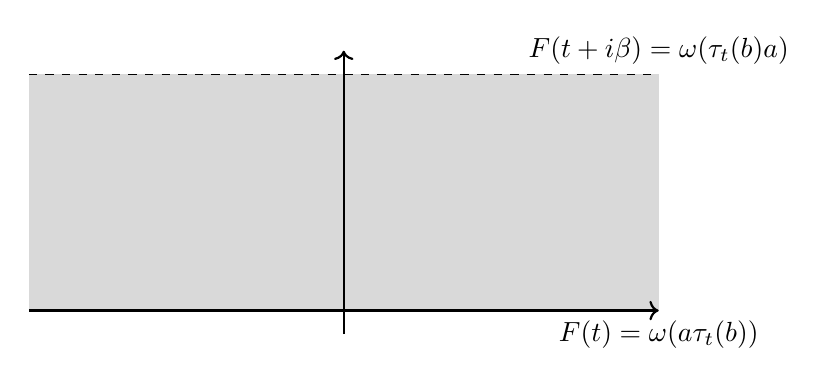
\begin{tikzpicture}
				\fill[gray!30] (-4,0) rectangle (4,3);
				\draw[->, thick] (-4,0) -- (4,0) node [below] {$F(t)=\omega(a\tau_t(b))$};
				\draw[->, thick] (0,-0.3) -- (0,3.3);
				\draw[dashed] (-4,3) -- (4,3) node [above] {$F(t+i\beta)=\omega(\tau_t(b)a)$};
			\end{tikzpicture}
		\end{figure}
	\end{definition}
\end{frame}

\begin{frame}
	\frametitle{KMS states as Equilibrium states}	
	KMS states are a candidate for a general definition of thermodynamic equilibrium in quantum systems\cite{Haag1967}:
	\begin{itemize}
		\item KMS states are invariant under the dynamics $\omega(\tau_t(a))=\omega(a)$;
		\item In finite dimensional Hilbert spaces with Schrödinger's time evolution $\tau$, the only possible $(\tau,\beta)$-KMS states are the $\beta$-Gibbs states
		\begin{align*}
			\mathcal{B}(\mathcal{H})&\rightarrow\mathbb{C} \\
			a&\mapsto \frac{\tr(ae^{-\beta H})}{\tr(e^{-\beta H})}.
		\end{align*}
		\item It is clear that the Gibbs prescription cannot be the characterization of equilibrium in the thermodynamic limit since coexistence of different phases demands that there cannot be a general unique correspondence between the Hamiltonian (evolution group) and states\cite{Connes1994}.
	\end{itemize}
\end{frame}

\section{Tomita-Takesaki Theory}

\begin{frame}
	\frametitle{Tomita-Takesaki Theory}
	For a $W^*$-algebra $\mathfrak{M}$ equipped with a cyclic and separating vector $\Omega$ the polar decomposition $S=J\Delta^{1/2}$ of the closure of
	\begin{align}
	\begin{split}
		S_0:\mathfrak{M}\Omega&\rightarrow\mathcal{H}\\
		A\Omega&\mapsto A^*\Omega
	\end{split}
	\end{align}
	yields:
	\begin{itemize}
		\item a one-parameter unitary group $t\mapsto\Delta^{it}$;
		\item a modular conjugation $J$.
	\end{itemize}
	\begin{theorem}[Tomita-Takesaki]
		\begin{itemize}
			\item $J\mathfrak{M}J=\mathfrak{M}'$;
			\item $\Delta^{it}\mathfrak{M}\Delta^{-it}=\mathfrak{M}$ for all $t\in\mathbb{R}$. 	
		\end{itemize}
	\end{theorem}
\end{frame}

\begin{frame}

	\frametitle{Modular Operators in Finite Dimensions}
	
	\begin{Example}
		In our previous example we have
		\begin{equation}
			S[a]=S\pi_\omega(a)[1]=\pi_\omega(a^*)[1]=[a^*].
		\end{equation}
From the action on the basis that diagonalizes the density operator
		\begin{equation}
			Se_i^{(\alpha)}=\frac{1}{\sqrt{\lambda_\alpha}}S[E_{i\alpha}]=\frac{1}{\sqrt{\lambda_\alpha}}[E_{\alpha i}]=\sqrt{\frac{\lambda_i}{\lambda_\alpha}}e_\alpha^{(i)}
		\end{equation}
We can obtain the polar decomposition by
		\begin{align}
		\begin{split}
			Je_i^{(\alpha)}=&e_\alpha^{(i)}\\
			\Delta e_i^{(\alpha)}=&\frac{\lambda_i}{\lambda_\alpha}e_i^{(\alpha)}
		\end{split}
		\end{align}
	\end{Example}

\end{frame}

\begin{frame}
	\frametitle{Modular Automorphism Group}
	\begin{definition}
		Let $\mathfrak{M}$ be a von Neumann algebra and $\omega$ be a faithful normal state. Due to $\bigstar$ we can perform the modular constructions on the cyclic representation $(\pi_\omega(\mathfrak{M}),\pi_\omega,\Omega_\omega)$. We define the modular automorphism group of $(\mathfrak{M},\omega)$ by 
		\begin{equation}
			\alpha_t(a)=\pi_\omega^{-1}(\Delta^{it}\pi_\omega(a)\Delta^{-it}).
		\end{equation}
	\end{definition}
	\begin{theorem}[$\bigstar\bigstar$]
		$(\mathfrak{M},\alpha)$ is a $W^*$-dynamical system  
	\end{theorem}		
	\begin{proof}
		\cite{Duvenhage1999}
	\end{proof}
\end{frame}

\begin{frame}

	\frametitle{Modular Automorphism Group in Finite Dimensions}
	
	\begin{Example}
		\begin{align}
		\begin{split}
			\Delta^{it}\pi_\omega(a)\Delta^{-it}e_i^{(\alpha)}=&\qty(\frac{\lambda_i}{\lambda_\alpha})^{-it}\sum_{k=1}^na_{ki}\qty(\frac{\lambda_k}{\lambda_\alpha})^{it}e_k^{(\alpha)}\\
			=&\sum_{k=1}^na_{ki}\qty(\frac{\lambda_k}{\lambda_i})^{it}e_k^{(\alpha)}\\
			=&\pi_\omega\qty(\sum_{i,k=1}^na_{ki}\qty(\frac{\lambda_k}{\lambda_i})^{it}E_{ki})e_i^{(\alpha)}.
		\end{split}
		\end{align}
		Therefore the modular automorphism group is
		\begin{equation}
			\alpha_t(a)=\sum_{i,j=1}^n\lambda_i^{it}a_{ij}\lambda_j^{-it}E_{ij}=\rho^{it}a\rho^{-it}
		\end{equation}
	\end{Example}

\end{frame}

\section{The Canonical Time Evolution}

\begin{frame}
	\frametitle{The Canonical Time Evolution}
	\begin{theorem}[$\bigstar\bigstar\bigstar$]
		Let $\mathfrak{M}$ be a von Neumann algebra and $\omega$ be a faithful normal state. Then $(\mathfrak{M},\tau)$ with $\tau_t(a) = \alpha_{-t/\beta}(a)$ and $\alpha$ the modular group of $(\mathfrak{M},\omega)$ is the unique $W^*$-dynamical system such that $\omega$ is a $(\tau,\beta)$-KMS state.
	\end{theorem}
	\begin{proof}
		\cite{Duvenhage1999}
	\end{proof}
\end{frame}

\begin{frame}

	\frametitle{Modular Hamiltonian in Finite Dimensions}
	
	\begin{Example}
		As we saw before
		\begin{equation}
			\tau_t(a)=\alpha_{-t/\beta}(a)=e^{iHt}ae^{-iHt}
		\end{equation}
where the modular Hamiltonian is given by
		\begin{equation}
			e^{iHt}=\rho^{-it/\beta}.
		\end{equation}
We conclude that indeed $\rho$ is a $\beta$-Gibbs state for this Hamiltonian!
		\begin{equation}
			\rho=e^{-\beta H}.
		\end{equation}
		
	\end{Example}

\end{frame}

\begin{frame}
	\frametitle{On von Neumann Algebras as Dynamical Objects}
	\begin{itemize}
		\item Through the modular group, states induce dynamics on the algebra of operators.
		\item The physical relevance of such prescription for evolution is guaranteed by the fact that it is the unique  dynamical law which makes the state an equilibrium state.
		\item One can use an analog of the Radon-Nikodym theorem to connect the modular groups induced by different states. Such a connection brings forward a canonical  homomorphism from $\mathbb{R}$ into the automorphism group of $\mathfrak{M}$ modulus inner automorphisms. This suggests that the emergence of the dynamical law might have a deeper origin.  
	\end{itemize}
\end{frame}

\begin{frame}[allowframebreaks]
	\frametitle{References}
	\bibliography{../Mendeley/library}
	\bibliographystyle{apalike}
\end{frame}

\end{document}